%% =============================================================================
%% Projeto Base - Artigo de TCC com abnTeX2
%% Customizado para a UNIJUÍ
%% Template desenvolvido e mantido por: Prof. Eldair F. Dornelles
%% A versão mais atualizada deste template pode ser obtida no GitHub:
%% https://github.com/dornelles/tcc-artigo-template-latex
%% Qualquer sugestão de melhoria será bem vinda, 
%% Contato pelo e-mail: eldair.dornelles@unijui.edu.br
%% =============================================================================

\documentclass[
    12pt,               % tamanho da fonte
    oneside,            % para impressão frente e verso (use oneside para apenas frente)
    a4paper,            % tamanho do papel
    chapter=TITLE,      % títulos de capítulos em maiúsculas
    section=TITLE,      % títulos de seções em maiúsculas
    english,            % idioma adicional para hifenização
    brazil,             % o último idioma é o principal do documento
    article             % formatação como artigo
]{abntex2}

% ==============================================================================
% PACOTES ESSENCIAIS
% ==============================================================================

% --- Codificação e fontes ---
\usepackage[T1]{fontenc}        % seleção de códigos de fonte
\usepackage[utf8]{inputenc}     % codificação do documento (conversão automática dos acentos)
% \usepackage{lmodern}          % comentado: a fonte agora está definida no arquivo unijui.sty

% --- Pacotes de citações ---
\usepackage[brazilian,hyperpageref]{backref}  % páginas com as citações na bibl
\usepackage[alf,bibjustif]{abntex2cite}        % citações padrão ABNT (bibjustif = referências justificadas)

% --- Pacotes matemáticos ---
\usepackage{amsmath}
\usepackage{amssymb}

% --- Pacotes gráficos ---
\usepackage{graphicx}           % inclusão de gráficos
% NOTA: NÃO usar \usepackage{float} com abnTeX2/memoir - conflita com \newfloat
\usepackage{subfig}             % subfiguras
\usepackage{pdfpages}           % inclusão de páginas PDF

% --- Pacotes de tabelas ---
\usepackage{booktabs}           % tabelas profissionais
\usepackage{multirow}           % células que ocupam várias linhas
\usepackage{longtable}          % tabelas longas (múltiplas páginas)
\usepackage{array}              % personalização de colunas

% --- Outros pacotes úteis ---
\usepackage{microtype}          % melhorias de justificação
\usepackage{indentfirst}        % indenta o primeiro parágrafo de cada seção
\usepackage{color}              % controle de cores
\usepackage{xcolor}             % cores avançadas
\newcommand{\pendente}[1]{\textcolor{red}{[#1]}} % marcação de trecho pendente no rascunho
\usepackage{listings}           % listagens de código-fonte
\usepackage{enumitem}           % listas personalizadas
\usepackage{lipsum}             % geração de texto fictício (remover na versão final)
\usepackage{totcount}           % conta o total de floats (figuras, tabelas, etc.) no documento

% --- Customizações UNIJUÍ ---
\input{unijui.sty}

% ==============================================================================
% CONFIGURAÇÕES DO PACOTE BACKREF
% ==============================================================================
% Configurações do pacote backref
% Usado sem a opção hyperpageref de backref
\renewcommand{\backrefpagesname}{Citado na(s) página(s):~}
% Texto padrão antes do número das páginas
\renewcommand{\backref}{}
% Define os textos da citação
\renewcommand*{\backrefalt}[4]{
    \ifcase #1 %
        Nenhuma citação no texto.%
    \or
        Citado na página #2.%
    \else
        Citado #1 vezes nas páginas #2.%
    \fi}%

% ==============================================================================
% CONFIGURAÇÕES DE LISTAGENS DE CÓDIGO
% ==============================================================================
\lstset{
    basicstyle=\ttfamily\small,
    numbers=left,
    numberstyle=\tiny\color{gray},
    stepnumber=1,
    numbersep=8pt,
    backgroundcolor=\color{white},
    showspaces=false,
    showstringspaces=false,
    showtabs=false,
    frame=single,
    rulecolor=\color{black},
    tabsize=2,
    captionpos=b,
    breaklines=true,
    breakatwhitespace=false,
    keywordstyle=\color{blue}\bfseries,
    commentstyle=\color{green!60!black},
    stringstyle=\color{red},
    escapeinside={\%*}{*)},
    literate=
        {á}{{\'a}}1 {é}{{\'e}}1 {í}{{\'i}}1 {ó}{{\'o}}1 {ú}{{\'u}}1
        {Á}{{\'A}}1 {É}{{\'E}}1 {Í}{{\'I}}1 {Ó}{{\'O}}1 {Ú}{{\'U}}1
        {ã}{{\~a}}1 {õ}{{\~o}}1 {Ã}{{\~A}}1 {Õ}{{\~O}}1
        {ç}{{\c{c}}}1 {Ç}{{\c{C}}}1
        {ê}{{\^e}}1 {â}{{\^a}}1 {ô}{{\^o}}1
}

% ==============================================================================
% DADOS DO TRABALHO
% ==============================================================================

% --- Informações do documento (preencher conforme o trabalho) ---

\titulo{Quão bons são os testes gerados por LLMs? Medindo a distância até o teto de qualidade alcançável}
% \subtitulo{Subtítulo (se houver)}

\tituloemingles{How good are LLM-generated tests? Measuring the distance to the attainable quality ceiling}
% \subtituloemingles{Subtitle (if any)}

\autor{Vítor Lewkowicz Klock}
\local{Santa Rosa/RS}
\data{2026}
\orientador{Prof. Junior Marcos Bandeira}
\instituicao{%
    Universidade Regional do Noroeste do\\[1mm]
    Estado do Rio Grande do Sul
}

% -- Autores para o artigo --
\autoresartigo{
    Vítor Lewkowicz Klock
    \thanks{Estudante do Curso de Engenharia de Software -- UNIJUÍ, Santa Rosa-RS, Brasil. E-mail: \texttt{vitor.klock@sou.unijui.edu.br}}
    \and
    Junior Marcos Bandeira
    \thanks{Professor Orientador -- UNIJUÍ, Santa Rosa-RS, Brasil. E-mail: \texttt{junior.bandeira@unijui.edu.br}}
}

% --- Informações específicas da UNIJUÍ (definidas no unijui.sty) ---
\campus{Santa Rosa}
\curso{Engenharia de Software}
\professordabanca{Prof(a). [membro da banca]}
\datadabanca{XX}{dezembro}{2026}

% --- Preâmbulo (texto da folha de rosto e aprovação) ---
% Não adicione ponto final do texto. Na folha de rosto o ponto irá aparecer automaticamente, 
% já na folha de aprovação ao invés de ponto irá aparecer uma vírgula, seguida do texto 
% "submetido à aprovação da banca examinadora composta pelos seguintes membros:"
\preambulo{Trabalho apresentado ao curso de Engenharia de Software da
            Universidade Regional do Noroeste do Estado do Rio Grande do Sul - UNIJUÍ,
            como requisito para a obtenção do título de Bacharel em Engenharia de Software}


% --- Texto de apresentação ---
\textoapresentacao{
    O presente trabalho está organizado no formato de artigo científico, conforme o modelo
    de Trabalho de Conclusão de Curso em formato de artigo adotado pelo curso de Engenharia
    de Software da UNIJUÍ. Após a defesa, pretende-se submetê-lo a um evento da Sociedade
    Brasileira de Computação, adaptando a formatação às normas do evento. \par
    O aparato experimental (código-alvo, prompts, suítes geradas, scripts de pontuação e
    resultados brutos) está disponível publicamente em:\\
    {\small\url{https://github.com/vitorklock/unijui-are-ai-tests-better-validator}}
}

% --- Resumo e Abstract ---
\resumoemportugues{%
   Modelos de linguagem de grande porte (LLMs) são usados rotineiramente para gerar testes de unidade, mas a qualidade do que geram costuma ser medida por cobertura, um indicador fraco de detecção de defeitos, ou comparada a testes humanos de qualidade desconhecida, e quase sempre a partir de uma única geração. Este trabalho propõe medir a distância até um teto de qualidade demonstrado: a melhor suíte que se consegue construir para o código-alvo com um desenvolvedor, uma LLM e ferramentas de mutação e de \textit{test smells}, iterando até que todo mutante sobrevivente tenha prova de equivalência. Para um avaliador de expressões em TypeScript com 369 mutantes, o teto ficou em 99,5\% de escore de mutação. Contra ele, medimos suítes geradas autonomamente por três LLMs (Claude Fable 5.1, Gemini 4 Neon e DeepSeek V4.1 Flash), com um prompt básico e um prompt ciente das métricas, em cinco gerações por condição, em cobertura, poder de detecção e densidade de \textit{smells}. Com o prompt básico, as suítes ficam a 3 pontos percentuais ou menos do teto em cobertura de linhas, mas a 8,4, 8,7 e 17,9 pontos em escore de mutação: executam quase tudo e verificam bem menos do que executam. O prompt ciente das métricas reduziu essa distância em 57\%, 75\% e 73\%, em todas as gerações, e colocou o modelo de baixo custo à frente dos modelos de fronteira sem orientação. A dispersão entre gerações variou de 0,4 a 2,5 pontos conforme o modelo, o suficiente para inverter a ordem entre condições vizinhas em até 36\% das amostras de geração única.
}
% Instrução: Use letras minúsculas para as palavras-chave, separe-as com ponto e vírgula (;) e encerre a última com um ponto (.)
\palavraschaveemportugues{geração de testes; modelos de linguagem; teste de mutação; qualidade de testes; test smells.}

\resumoemingles{
   Large language models (LLMs) are routinely used to generate unit tests, yet the quality of what they produce is usually measured by coverage, a weak indicator of fault detection, or compared against human-written tests of unknown quality, and almost always from a single generation. This work proposes measuring the distance to a demonstrated quality ceiling: the best test suite that can be built for the target with a developer, an LLM and mutation and test-smell tools, iterating until every surviving mutant has a proof of equivalence. For a TypeScript expression evaluator with 369 mutants, the ceiling reached a 99.5\% mutation score. Against it, we measured suites generated autonomously by three LLMs (Claude Fable 5.1, Gemini 4 Neon and DeepSeek V4.1 Flash), with a basic prompt and a metrics-aware prompt, in five generations per condition, on coverage, fault-detection power and smell density. With the basic prompt, suites fall within 3 percentage points of the ceiling in line coverage but 8.4, 8.7 and 17.9 points below it in mutation score: they execute almost everything and verify far less than they execute. The metrics-aware prompt reduced that distance by 57\%, 75\% and 73\%, in every generation, and placed the low-cost model ahead of the frontier models without guidance. Dispersion across generations ranged from 0.4 to 2.5 points depending on the model, enough to invert the order of neighbouring conditions in up to 36\% of single-generation samples.
}
% Instruction: Use lowercase letters for keywords, separate them with semicolons (;) and end the last one with a period (.).
\palavraschaveemingles{test generation; large language models; mutation testing; test quality; test smells.}




% ==============================================================================
% CONFIGURAÇÕES DE APARÊNCIA DO PDF FINAL
% ==============================================================================
\makeatletter
\hypersetup{
    pdftitle={\@title},
    pdfauthor={\@author},
    pdfsubject={\imprimirpreambulo},
    pdfcreator={LaTeX com abnTeX2},
    pdfkeywords={geração de testes}{LLM}{teste de mutação}{qualidade de testes}{test smells},
    colorlinks=true,        % false: links em caixas; true: links coloridos
    linkcolor=black,        % cor dos links internos
    citecolor=black,        % cor dos links para bibliografias
    filecolor=black,        % cor dos links de arquivos
    urlcolor=black,         % cor dos links de URLs
    bookmarksdepth=4
}
\makeatother

% ==============================================================================
% ESPAÇAMENTOS ENTRE LINHAS E PARÁGRAFOS
% ==============================================================================
% O tamanho do parágrafo é dado por:
\setlength{\parindent}{1.3cm}
% Controle do espaçamento entre um parágrafo e outro:
\setlength{\parskip}{0.2cm}  % tente também \onelineskip



% ==============================================================================
% INÍCIO DO DOCUMENTO
% ==============================================================================
\begin{document}

% Seleciona o idioma do documento
\selectlanguage{brazil}

% Retira espaço extra obsoleto entre as frases
\frenchspacing

% --- Imprimir página de créditos e marca d'água ---
% \imprimirpaginadecreditos
% \imprimirmarcadagua

% ==========================================================================
% ELEMENTOS PRÉ-TEXTUAIS
% ==========================================================================
\pretextual

% --- Capa ---
\imprimircapa

% --- Folha de rosto ---
% (o * indica que haverá a ficha bibliográfica)
\imprimirfolhaderosto

% --- Ficha catalográfica (inserir PDF gerado pela biblioteca) ---
% \begin{fichacatalografica}
%     \includepdf{fig_ficha_catalografica.pdf}
% \end{fichacatalografica}

% --- Folha da banca ---
\imprimirfolhadabanca

% --- Agradecimentos ---
% \begin{agradecimentos}
%     [Agradecimentos: opcional; preencher se desejar.]
% \end{agradecimentos}
% \newpage


% --- Lista de ilustrações (só aparece se houver figuras) ---
% Na primeira compilação os contadores podem ser 0; compile 2x para resultado correto.
\ifnum\totvalue{figcount}>0
    \pdfbookmark[0]{\listfigurename}{lof}
    \listoffigures*
    \cleardoublepage
    \newpage
\fi

% --- Lista de quadros (só aparece se houver quadros) ---
\ifnum\totvalue{quacount}>0
    \pdfbookmark[0]{\listofquadrosname}{loq}
    \listofquadros*
    \cleardoublepage
    \newpage
\fi

% --- Lista de tabelas (só aparece se houver tabelas) ---
\ifnum\totvalue{tabcount}>0
    \pdfbookmark[0]{\listtablename}{lot}
    \listoftables*
    \cleardoublepage
    \newpage
\fi

% --- Lista de abreviaturas e siglas ---
\begin{siglas}
    \item[API] \textit{Application Programming Interface}
    \item[AST] \textit{Abstract Syntax Tree} (árvore sintática abstrata)
    \item[FP] Falso positivo
    \item[IC] Intervalo de confiança
    \item[LLM] \textit{Large Language Model} (modelo de linguagem de grande porte)
    \item[QP] Questão de pesquisa
    \item[SBC] Sociedade Brasileira de Computação
    \item[TCC] Trabalho de Conclusão de Curso
    \item[UNIJUÍ] Universidade Regional do Noroeste do Estado do Rio Grande do Sul
\end{siglas}


% --- Sumário ---
\pdfbookmark[0]{\contentsname}{toc}
\tableofcontents*
\cleardoublepage


% --- Página de Apresentação ---
\begin{apresentacao}
    \imprimirapresentacao
\end{apresentacao}
\newpage

% --- Página de Resumo e Abstract ---
\imprimirpaginaresumos


% ==========================================================================
% ELEMENTOS TEXTUAIS
% ==========================================================================
\textual

% --- Inclusão dos capítulos ---
% ==============================================================================
% 1. INTRODUÇÃO
% ==============================================================================
\chapter{Introdução}
\label{cap:introducao}

Testar software custa caro e, ainda assim, costuma ser a parte do trabalho que fica para depois. O relatório clássico do NIST estimou em dezenas de bilhões de dólares por ano o prejuízo causado por infraestrutura inadequada de testes nos Estados Unidos \cite{tassey2002}, e a dificuldade de escrever bons testes continua sendo uma das razões pelas quais muitos projetos simplesmente não os têm \cite{siddiq2024}. Nesse cenário, assistentes de programação baseados em modelos de linguagem de grande porte (LLMs) entraram rápido no dia a dia dos desenvolvedores \cite{liang2024}, e gerar testes de unidade é uma das tarefas que mais se delega a eles: basta apontar o modelo para o código e pedir ``escreva os testes''.

A pergunta que interessa é o que se recebe de volta. A literatura sobre geração de testes com LLMs cresceu depressa, mas a forma de medir a qualidade do que é gerado ainda é frágil em dois pontos. O primeiro é a métrica: boa parte dos estudos reporta cobertura de código, que é fácil de medir mas é um indicador fraco da capacidade de detectar defeitos \cite{inozemtseva2014}; uma suíte pode executar todas as linhas e não falhar quando a lógica muda, porque suas asserções são frouxas. O segundo é a linha de base: quando há comparação, ela é feita contra testes escritos por humanos cuja qualidade raramente é conhecida. \citeonline{walczak2025}, por exemplo, usam como referência a suíte de um praticante que atinge 98\% de cobertura de ramos e apenas 44\% de escore de mutação, e concluem que várias configurações de LLM a superam. Superar uma suíte mediana diz pouco sobre o quanto falta para uma suíte boa.

Há ainda um terceiro problema, mais silencioso. LLMs são não determinísticos: o mesmo prompt produz saídas diferentes a cada chamada, e \citeonline{ouyang2025} mostram que, em geração de código, a fração de tarefas em que nenhuma das respostas repetidas produz a mesma saída chega a três quartos. Mesmo assim, a prática comum em avaliações de geração de testes é medir uma única geração por condição e tratar o número obtido como ``o'' resultado daquele modelo. Não se sabe quanto desse número é propriedade do modelo e quanto é sorte de amostragem.

Este trabalho propõe medir a qualidade dos testes gerados por LLMs de outro jeito: pela \textbf{distância até um teto de qualidade demonstrado}. O teto é a melhor suíte de testes que se consegue construir para o código-alvo usando todos os recursos disponíveis (um desenvolvedor experiente, a melhor LLM que tínhamos, e ferramentas de análise de mutação e de \textit{smells}) iterando até que o escore de mutação sature e cada mutante sobrevivente tenha uma prova de que é equivalente ou inalcançável. Contra esse teto, medimos suítes geradas de forma autônoma por três LLMs atuais, em duas condições de prompt, com cinco gerações independentes por condição. A qualidade é medida em três dimensões: cobertura (linhas e ramos), poder de detecção de defeitos (escore de mutação, lido como \textit{recall}, e precisão, lida a partir dos testes que falham sobre o código correto) e manutenibilidade (densidade de \textit{test smells}).

As questões de pesquisa são:

\begin{description}
    \item[QP1.] Dado um teto de qualidade demonstrado para o código-alvo, a que distância dele ficam as suítes geradas autonomamente por LLMs, em cada dimensão?
    \item[QP2.] Um prompt que informa à LLM os critérios pelos quais os testes serão avaliados reduz essa distância?
    \item[QP3.] Em qual dimensão a distância é maior?
    \item[QP4.] Quão estável é a distância entre gerações repetidas da mesma condição? Uma única geração basta para caracterizá-la?
\end{description}

As contribuições são: (i) um método de avaliação baseado em teto demonstrado, com aparato de replicação público; (ii) um teto construído e revisado para um avaliador de expressões em TypeScript com 369 mutantes, no qual os oito mutantes que restam vivos têm prova de equivalência ou de inalcançabilidade; (iii) medições de distância, com repetição, para três modelos atuais e dois prompts; (iv) evidência sobre quanto uma avaliação de geração única pode ser confiada; e (v) um achado metodológico sobre a pontuação de mutação executada em paralelo, que inflou o escore do próprio teto em 2,4 pontos percentuais por meio de \textit{timeouts} espúrios.

O restante do texto está organizado assim: o \autoref{cap:metodologia} descreve o desenho do estudo, as variáveis, os procedimentos e a análise; o \autoref{cap:referencial} situa cobertura, teste de mutação, \textit{test smells}, geração de testes com LLMs e não determinismo; o \autoref{cap:desenvolvimento} apresenta o código-alvo, o aparato, a construção do teto, as condições experimentais, os resultados, a discussão e as ameaças à validade; e o \autoref{cap:consideracoes} fecha com as respostas às questões e os próximos passos.

% ==============================================================================
% 2. METODOLOGIA
% ==============================================================================
\chapter{Metodologia}
\label{cap:metodologia}

\section{Classificação da pesquisa}

Quanto à natureza, esta é uma pesquisa aplicada: o problema é prático (saber o que se recebe ao pedir testes a uma LLM) e o resultado se destina a quem usa essas ferramentas e a quem as avalia. Quanto à abordagem, é quantitativa: todas as variáveis de resposta são medidas por instrumentação, sem julgamento humano na pontuação. Quanto aos objetivos, é explicativa, no sentido de \citeonline{gil2017}, porque isola fatores (modelo, prompt, repetição) e mede o efeito de cada um sobre a distância até o teto. Quanto aos procedimentos, é um experimento controlado, nos termos de \citeonline{wohlin2012}: um objeto fixo, fatores manipulados com níveis definidos, variáveis de resposta medidas da mesma forma em todas as condições e repetições independentes para estimar a variação.

O estudo não parte de uma base de dados existente. Os dados são as métricas de qualidade que a instrumentação produz ao avaliar cada suíte de teste; cada execução de uma suíte sobre o código-alvo rende uma linha de medições.

\section{Objeto, fatores e repetições}

O objeto de estudo é um avaliador de expressões em TypeScript, descrito na seção ``\nameref{sec:alvo}'', fixo em todo o experimento; o Stryker gera para ele 369 mutantes válidos. Há dois fatores manipulados. O fator \textbf{modelo} tem três níveis, escolhidos para cobrir faixas distintas de custo e capacidade: dois modelos de fronteira, um acessado por ferramenta de codificação e outro por aplicativo de chat, e um modelo de baixo custo acessado por API (seção ``\nameref{sec:condicoes}''). O fator \textbf{prompt} tem dois níveis: P1, um pedido básico de testes, e P2, o mesmo pedido acrescido dos critérios pelos quais a suíte será avaliada (Apêndice~\ref{ap:prompts}). Cada combinação modelo~$\times$~prompt é uma \textbf{condição}, e cada condição é gerada $k = 5$ vezes, de forma independente, totalizando 30 suítes. A referência é o \textbf{teto de qualidade}, uma suíte única construída e revisada conforme a seção ``\nameref{sec:teto}''.

A escolha de $k = 5$ é um compromisso entre o custo de gerar e pontuar cada suíte e a necessidade de ter, para cada condição, uma estimativa de dispersão e não só um ponto. A QP4 avalia, a partir da dispersão observada, se esse $k$ é suficiente e quanto seria necessário para uma precisão alvo.

\section{Variáveis de resposta e métricas}
\label{sec:metricas}

Cada suíte é medida nas mesmas seis variáveis, agrupadas em três dimensões:

\begin{enumerate}
    \item \textbf{Cobertura.} Cobertura de linhas (Cob.L) e de ramos (Cob.R), em porcentagem, medidas pelo Vitest com o provedor V8 sobre os três arquivos de lógica do alvo.
    \item \textbf{Poder de detecção de defeitos.} Tratamos cada caso de teste como um detector. O \textit{recall} $R$ é o escore de mutação:
    \begin{equation}
        R = \frac{M_{\text{mortos}} + M_{\text{timeout}}}{M_{\text{válidos}}},
        \label{eq:recall}
    \end{equation}
    em que $M_{\text{válidos}}$ exclui mutantes com erro de compilação ou de execução. A precisão $P$ é a fração dos casos de teste que passam sobre o código correto:
    \begin{equation}
        P = \frac{T - \text{FP}}{T},
        \label{eq:precisao}
    \end{equation}
    em que $T$ é o número de casos de teste e FP é o número deles que falham sobre o código correto (um falso positivo: o teste acusa um defeito que não existe). $F_1$ é a média harmônica de $P$ e $R$.
    \item \textbf{Manutenibilidade.} Densidade de \textit{test smells}: ocorrências detectadas pelos 15 detectores do SNUTS.js \cite{oliveira2024snuts} divididas pelo número de casos de teste.
\end{enumerate}

A variável de interesse é a \textbf{distância até o teto}, calculada por métrica:
\begin{equation}
    \Delta_m = m_{\text{teto}} - m_{\text{suíte}},
    \label{eq:gap}
\end{equation}
positiva quando a suíte fica abaixo do teto (para densidade de \textit{smells}, em que menor é melhor, o sinal é invertido para manter a leitura ``positivo é pior''). Para cada condição reportamos média, desvio padrão, mínimo e máximo das cinco gerações.

Duas decisões sobre as métricas merecem registro. A primeira: o StrykerJS não identifica mutantes equivalentes, então eles permanecem no denominador da \autoref{eq:recall} para \textbf{todas} as suítes, teto incluído; o $R$ reportado é um limite inferior do escore ``verdadeiro'', mas a comparação entre teto e LLMs é feita numa única definição. A segunda: suítes são pontuadas exatamente como geradas, sem correção. Testes que falham sobre o código correto contam como FP e reduzem $P$; apenas na execução de mutação eles são desativados, porque um teste que já falha sobre o código original não é um detector válido e impediria a linha de base verde do Stryker. Corrigir a saída da LLM antes de medi-la contaminaria a medida de qualidade \textit{autônoma}, que é o que se quer medir.

\section{Procedimentos}

O experimento tem quatro etapas. \textbf{(1) Construção e revisão do teto.} A suíte de referência foi construída iterativamente, sem restrição de meios: escrita inicial com apoio de LLM, leitura do relatório de mutação, novos testes para cada mutante sobrevivente, remoção de \textit{smells}, nova rodada, até o escore saturar. Em seguida, cada mutante ainda vivo foi analisado manualmente e classificado como matável (e então morto) ou equivalente, com argumento de por que nenhum teste válido o distingue do original. O critério é o do teste de mutação, não o da API: um mutante em código que nenhuma entrada alcança ainda é matável se um teste puder alcançá-lo por injeção de dependência. O teto só é considerado pronto quando não resta mutante matável, e qualquer suíte gerada que o supere em qualquer métrica reabre a revisão. \textbf{(2) Geração das suítes.} Cada geração parte de uma cópia limpa do projeto-alvo, em diretório neutro, sem histórico, sem os prompts e sem vestígio do aparato de avaliação. A LLM recebe uma única mensagem (o prompt da condição e, para os modelos sem acesso ao sistema de arquivos, o conteúdo dos arquivos do projeto) e devolve o arquivo de testes; não há segunda mensagem, execução de testes com retorno para o modelo nem correção, e a saída é salva como veio. Memória e personalização dos aplicativos ficam desligadas, e cada repetição usa uma sessão nova. \textbf{(3) Pontuação.} Cada suíte é copiada para um ambiente isolado com o código-alvo e pontuada por um único \textit{script}: execução com cobertura e registro de falhas por caso de teste; desativação dos FP; execução do Stryker; contagem de \textit{smells}; cálculo das métricas e das distâncias. Toda a pontuação é \textbf{sequencial}, uma suíte por vez, num mesmo ambiente, pelo motivo descrito na seção ``\nameref{sec:aparato}''. \textbf{(4) Análise.} Para QP1 a QP3, estatística descritiva das distâncias por condição e por dimensão, com intervalos de confiança de 95\% por \textit{bootstrap} percentil (10\,000 reamostragens) sobre as cinco gerações; para o efeito do prompt (QP2), o \textit{delta} de Cliff entre P2 e P1 em cada modelo. Para QP4, desvio padrão e coeficiente de variação entre gerações por condição; a frequência com que o ordenamento das condições pela média se mantém ao tomar uma geração ao acaso por condição; e o número de gerações necessário para que a semi-amplitude do intervalo de 95\% fique em 2 pontos percentuais, por $n = (1{,}96\,s/E)^2$. Com $k = 5$ não há poder para testes de hipótese convencionais, e não os fazemos.

\section{Instrumentos e reprodutibilidade}

O aparato é composto por dois repositórios: o \texttt{bench}, com o código-alvo e uma configuração mínima do Vitest, que é tudo o que uma LLM vê; e o \texttt{validator}, com os prompts, a suíte do teto, as suítes geradas, os \textit{scripts} de geração e de pontuação, a configuração do StrykerJS (8.7, com executor do Vitest 1.6 e cobertura por teste) e os detectores do SNUTS.js. O estudo não envolve participantes humanos. Todos os artefatos, incluindo as respostas completas dos modelos e os resultados em JSON, estão públicos no repositório indicado na apresentação.

% ==============================================================================
% 3. REFERENCIAL TEÓRICO
% ==============================================================================
\chapter{Referencial teórico}
\label{cap:referencial}

\section{Cobertura e suas limitações}

Critérios de cobertura medem quanto do programa uma suíte exercita: linhas, ramos, condições \cite{ammann2016}. São baratos de medir e fáceis de comunicar, e por isso viraram a métrica padrão de ``qualidade de testes'' em ferramentas, em equipes e em boa parte da pesquisa. O problema é que cobertura mede execução, não verificação. Um teste que chama uma função e não afirma nada sobre o resultado cobre as mesmas linhas que um teste que afirma o valor exato. \citeonline{inozemtseva2014} mediram, em projetos Java de tamanhos variados, a correlação entre cobertura e a capacidade da suíte de detectar defeitos, e encontraram correlação fraca a moderada, que desaparece quando se controla pelo número de testes. A conclusão deles é direta: cobertura indica o que \textit{não} foi testado, mas uma cobertura alta não é evidência de que o que foi testado está bem testado.

\section{Teste de mutação}

Teste de mutação inverte a pergunta. Em vez de medir o que a suíte executa, mede o que ela detecta. A ideia, formulada por \citeonline{demillo1978}, é introduzir pequenas alterações sintáticas no programa (os \textit{mutantes}: trocar \texttt{<} por \texttt{<=}, negar uma condição, remover uma instrução) e rodar a suíte contra cada versão alterada. Se algum teste falha, o mutante foi \textit{morto}; se todos passam, ele \textit{sobreviveu}, e a suíte não distingue o programa original daquela variante. O escore de mutação é a fração de mutantes mortos. A hipótese do programador competente e o efeito de acoplamento, discutidos em detalhe na revisão de \citeonline{papadakis2019}, justificam por que alterações pequenas servem como substitutos de defeitos reais, e \citeonline{just2014} deram suporte empírico a isso ao mostrar, com 357 defeitos reais, que suítes que matam mais mutantes também detectam mais defeitos reais, de forma independente da cobertura.

Dois detalhes práticos importam para este trabalho. O primeiro são os \textbf{mutantes equivalentes}: alterações que não mudam o comportamento observável do programa (por exemplo, trocar o valor inicial de uma variável que é sempre reatribuída antes de ser lida). Nenhum teste consegue matá-los, e a decisão de equivalência é, no caso geral, indecidível \cite{papadakis2019}; ferramentas não os identificam, e eles ficam no denominador, rebaixando o escore máximo atingível. O segundo são os \textbf{\textit{timeouts}}: quando um mutante faz o programa não terminar (um laço cuja condição de parada foi alterada), a ferramenta interrompe a execução após um limite de tempo e conta o mutante como detectado. Esse limite é calculado a partir do tempo de uma execução de referência, e por isso é sensível à carga da máquina. O StrykerJS \cite{stryker}, usado aqui, implementa operadores para JavaScript e TypeScript, integra-se ao Vitest \cite{vitest} e reporta separadamente mutantes mortos, sobreviventes, por \textit{timeout} e sem cobertura.

\section{\textit{Test smells}}

Testes também são código, e código que vai ser mantido. \citeonline{vandeursen2001} cunharam o termo \textit{test smell} para padrões em código de teste que dificultam entender, manter e confiar nos testes: o \textit{Assertion Roulette} (várias asserções sem mensagem num mesmo teste, de modo que não se sabe qual falhou), o \textit{Eager Test} (um teste que verifica vários comportamentos de uma vez), o \textit{Mystery Guest} (dependência de recursos externos ao teste), entre outros. \citeonline{meszaros2007} sistematizou esses padrões e os remédios correspondentes. Para JavaScript e TypeScript, o SNUTS.js \cite{oliveira2024snuts} detecta quinze \textit{smells} por análise da árvore sintática do arquivo de teste, o que permite medir manutenibilidade de forma automática e reprodutível. \citeonline{siddiq2024} encontraram \textit{smells} como asserções duplicadas e testes vazios em suítes geradas por LLMs, o que motiva incluir essa dimensão na avaliação.

\section{Geração de testes com LLMs e suas linhas de base}

A geração automática de testes antecede as LLMs: ferramentas baseadas em busca, como o EvoSuite, maximizam cobertura por algoritmos evolutivos, e \citeonline{lemieux2023} mostraram que uma LLM pode ajudar essas ferramentas a escapar de platôs de cobertura. Com modelos de propósito geral, a geração direta a partir de um prompt se tornou viável. \citeonline{schafer2024} avaliaram essa abordagem em 25 pacotes JavaScript e obtiveram cobertura mediana de instruções de 70\%, com uma fração relevante de testes que falhavam ou não compilavam. \citeonline{yuan2024} analisaram testes gerados pelo ChatGPT para Java e encontraram cobertura comparável à de ferramentas tradicionais, mas problemas frequentes de correção, que motivaram um processo iterativo de correção guiado por feedback do compilador e do executor. \citeonline{siddiq2024} chegaram a conclusões semelhantes para três modelos de código.

Há duas lacunas nesses estudos que este trabalho tenta fechar. A primeira é a \textbf{linha de base}. Quando há comparação, ela é feita contra testes escritos por humanos, tomados como padrão-ouro: o \textit{benchmark} TestGenEval \cite{jain2025testgeneval}, por exemplo, mede cobertura e escore de mutação dos testes gerados em relação aos testes humanos do próprio repositório, e \citeonline{walczak2025} usam a suíte de um praticante com 44\% de escore de mutação. Suítes humanas são úteis como referência do que se faz na prática, mas não do que é possível fazer; concluir que uma LLM ``supera o humano'' contra essa referência não diz quanto falta para uma suíte realmente boa. A segunda lacuna é o \textbf{oráculo}: \citeonline{konstantinou2024} mostram que oráculos gerados por LLMs tendem a capturar o comportamento real do código, e não o pretendido, o que limita a detecção de defeitos lógicos. O escore de mutação é a métrica certa para expor isso, porque mutantes são justamente desvios do comportamento real que uma asserção frouxa deixa passar. \citeonline{wang2025mutgen} usam mutação dentro do laço de geração, realimentando a LLM com os mutantes vivos; o uso aqui é diferente: a mutação é o juiz externo, não parte da geração, e a referência é um teto maximizado, não uma suíte humana.

\section{Não determinismo}

LLMs amostram tokens de uma distribuição de probabilidade; a mesma entrada gera saídas diferentes a cada chamada, e isso não é um detalhe de configuração. \citeonline{ouyang2025} estudaram o fenômeno em geração de código com 829 problemas e observaram que, na configuração padrão, a fração de tarefas em que nenhuma das execuções repetidas produz a mesma saída de teste foi de 75,8\%, 51,0\% e 47,6\% em três \textit{benchmarks}, e que fixar a temperatura em zero reduz, mas não elimina, a variação. Os autores alertam que isso é uma ameaça à validade de conclusão de qualquer estudo que compare modelos a partir de uma única execução. Para avaliação de testes gerados, a implicação é concreta: um escore de mutação medido uma vez é uma amostra de tamanho um de uma variável aleatória cuja dispersão ninguém mediu. A QP4 deste trabalho mede essa dispersão.

% ==============================================================================
% 4. DESENVOLVIMENTO
% ==============================================================================
\chapter{Desenvolvimento}
\label{cap:desenvolvimento}

\section{Código-alvo}
\label{sec:alvo}

O código-alvo é um avaliador de expressões em TypeScript, escrito para suportar cláusulas no estilo do \texttt{WHERE} do SQL: comparações (\texttt{=}, \texttt{<>}, \texttt{<}, \texttt{<=}, \texttt{>}, \texttt{>=}), aritmética (\texttt{+}, \texttt{-}, \texttt{*}, \texttt{/}), operadores lógicos (\texttt{and}, \texttt{or}), \texttt{is [not] null}, \texttt{between}, expressões \texttt{case when \ldots then \ldots else \ldots end}, chamadas de função (\texttt{length}), literais numéricos, de texto e booleanos, identificadores resolvidos por um contexto e agrupamento por parênteses. Ele tem 622 linhas em cinco arquivos: \texttt{lexer.ts} (206 linhas), que converte o texto em \textit{tokens}; \texttt{parser.ts} (221), um \textit{parser} de precedência de operadores que produz uma árvore sintática; \texttt{evaluator.ts} (89), que percorre a árvore e calcula o valor; e \texttt{ast.ts} (52) e \texttt{token.ts} (54), que só definem tipos. A API pública tem três funções: \texttt{parse(expression)}, \texttt{evaluate(expression, context?)} e \texttt{evaluateObject(expression, value)}.

A escolha é deliberada. O alvo é lógica pura e determinística, sem E/S, sem dependências e sem estado compartilhado, o que elimina fontes de variação alheias à suíte. É pequeno o bastante para que um teto possa ser construído e \textbf{demonstrado} (cada mutante sobrevivente pode ser analisado um a um), e rico o bastante para ser difícil de testar bem: há precedência de operadores, fronteiras de classes de caracteres no \textit{lexer}, tratamento de fim de entrada, mensagens de erro com posição e vários caminhos de erro sintático. O StrykerJS gera 369 mutantes válidos nos três arquivos de lógica (177 no \textit{lexer}, 92 no \textit{parser}, 100 no avaliador), dominados por expressões condicionais (138), remoção de blocos (77), literais de texto (50) e operadores de igualdade (47).

\section{Aparato de avaliação}
\label{sec:aparato}

O aparato separa o que a LLM vê do que a julga. O repositório \texttt{bench} contém apenas o código-alvo, um \texttt{package.json} com o Vitest e uma configuração mínima de teste; é um projeto comum que precisa de testes. O repositório \texttt{validator} contém tudo o mais: os prompts, a suíte do teto, cada suíte gerada, o \textit{script} de pontuação, a configuração do Stryker e os detectores do SNUTS.js. Um \textit{script} verifica, por \textit{hash}, que o código mutado é byte a byte o mesmo que a LLM testou. Antes de cada geração, o \texttt{bench} é copiado para um diretório com nome neutro e sem histórico, para que nem o caminho nem o \texttt{git log} revelem que existe um avaliador.

A pontuação de uma suíte segue sempre o mesmo caminho: (1) o Vitest executa a suíte sobre o código correto, com cobertura por V8 restrita aos três arquivos de lógica e com emissão de cobertura mesmo quando há falhas, e registra quais casos de teste falharam; (2) os casos que falharam são marcados como ignorados numa cópia da suíte, usada apenas na etapa seguinte; (3) o StrykerJS roda a cópia contra os 369 mutantes, com análise de cobertura por teste; (4) os detectores do SNUTS.js contam \textit{smells} na suíte original; (5) as métricas da seção ``\nameref{sec:metricas}'' e as distâncias até o teto são calculadas e gravadas em JSON. Nada é corrigido à mão em nenhuma etapa.

\subsection{Um achado sobre a execução em paralelo}
\label{sec:timeout}

A primeira versão do \textit{script} pontuava várias suítes ao mesmo tempo, cada uma com seu próprio processo do Stryker, que por sua vez abre vários processos de trabalho. Numa rodada-piloto com seis suítes de modelos anteriores, executada assim, o teto de então marcou 95,1\% de escore de mutação. Pontuado de novo, sozinho, no mesmo ambiente, ele marcou 92,7\%. A diferença estava inteiramente nos \textit{timeouts}: 95 mutantes na execução paralela contra 29 na sequencial. O Stryker calcula o tempo-limite de cada mutante a partir de uma execução de referência; quando a máquina está sob carga, mutantes que apenas tornam o código mais lento, sem impedir que termine, estouram o limite e são contados como mortos. Nas seis suítes de LLM do piloto, repontuadas em sequência, a inflação variou de 0,5 a 5,4 pontos percentuais e não foi uniforme: a distância de uma mesma suíte até o teto, que era de 5,1 pontos na pontuação paralela, passou a 13,3 pontos na sequencial, porque teto e suíte tinham sido inflados em medidas diferentes.

A consequência prática é que escores de mutação obtidos em execuções paralelas não são comparáveis entre si nem com execuções isoladas, e são sistematicamente otimistas. Toda a pontuação deste estudo é sequencial, e as tabelas reportam mutantes mortos e por \textit{timeout} em colunas separadas. Os 29 \textit{timeouts} que restam na execução sequencial correspondem a mutações que de fato removem a condição de parada de laços do \textit{lexer} e do \textit{parser}, e são detecções legítimas.

\section{Construção e revisão do teto}
\label{sec:teto}

O teto foi construído em duas fases. Na primeira, uma suíte foi escrita com apoio de LLM e refinada a partir dos relatórios do Stryker e do SNUTS.js até o escore saturar, chegando a 104 testes, cobertura de 99,2\% de linhas e 97,3\% de ramos, nenhum \textit{smell} e, medida sequencialmente, 92,7\% de escore de mutação, com 21 mutantes sobreviventes e 6 sem cobertura.

Na segunda fase, cada um desses 27 mutantes foi analisado individualmente. O resultado mudou a leitura do que a primeira fase tinha produzido: dos 21 sobreviventes, 19 eram matáveis. Eram, quase todos, casos de fronteira que a suíte original não exercitava: o dígito \texttt{9}, limite superior da faixa numérica do \textit{lexer} (a suíte usava 0 a 8 e não percebia que a mutação \texttt{<= 0x39} $\to$ \texttt{< 0x39} tornava \texttt{9} um caractere ilegal); um número decimal com mais de um dígito antes do ponto (\texttt{12.5}), porque com um dígito só a mutação na guarda do ponto decimal é indistinguível; identificadores começando por \texttt{A}, \texttt{Z} e \texttt{z}, os limites das faixas de letras; os caracteres \texttt{[} e \texttt{\{}, imediatamente após \texttt{Z} e \texttt{z}, que devem ser ilegais; o cálculo da posição do \textit{token}, que só é observável nas mensagens de erro e que a suíte verificava com expressões regulares parciais; e a guarda de \texttt{case} sem \texttt{when}, que só é distinguível com a entrada \texttt{case end}. Doze testes, um comportamento por teste, mataram os 19. A suíte final tem 116 testes, 97,8\% de escore de mutação (332 mutantes mortos, 29 por \textit{timeout}, 2 sobreviventes, 6 sem cobertura), mesma cobertura e nenhum \textit{smell}.

Os oito mutantes restantes têm, cada um, um argumento de por que nenhum teste pode matá-los, registrado no Apêndice~\ref{ap:equivalentes}. Dois são equivalentes no sentido clássico: o valor inicial de um campo que o construtor reatribui antes de qualquer leitura, e o valor de fim de entrada devolvido por \texttt{peekChar}, que só é usado em comparações nas quais \texttt{""} e \texttt{'\textbackslash 0'} se comportam igual. Seis são código inalcançável pela API pública: um \texttt{if} cuja condição nunca é verdadeira porque a função chamada retorna um objeto ou lança exceção, e dois ramos \texttt{default} de \textit{switches} para operadores e tipos de nó que o \textit{parser} nunca produz. As linhas não cobertas pela suíte (99,2\% de linhas) são exatamente essas, então a cobertura do teto também é a máxima alcançável pela API pública. Subtraindo os oito do denominador, o teto atinge 100\%; mantendo-os, como fazemos para todas as suítes, 97,8\% é o limite superior para este alvo.

Duas lições ficam dessa fase. A primeira é que uma suíte construída com LLM, ferramentas e iteração, e que parecia saturada, ainda deixava 19 mutantes matáveis em fronteiras de classes de equivalência; o que a tornou um teto não foi o processo de construção, foi a análise individual dos sobreviventes. A segunda é que ``teto'' é uma afirmação sobre o alvo, não sobre quem o construiu, e por isso ela precisa vir acompanhada de prova: sem a classificação dos sobreviventes, qualquer distância medida contra a referência carrega uma incerteza que não se consegue quantificar.

\section{Condições experimentais e geração}
\label{sec:condicoes}

A \autoref{tab:modelos} lista os modelos. Os três foram usados na mesma condição de interface: uma única mensagem contendo o prompt da condição e o projeto-alvo, sem execução de testes, sem segunda rodada e sem correção. Para o modelo acessado por ferramenta de codificação, isso foi obtido executando a ferramenta em modo não interativo com as ferramentas de leitura e escrita de arquivos habilitadas e a execução de comandos desabilitada: o modelo lê os arquivos do projeto e escreve o arquivo de testes, e só. Para o modelo acessado por aplicativo de chat e para o acessado por API, o conteúdo dos cinco arquivos do projeto e da configuração do Vitest foi incluído na própria mensagem, logo após o prompt, com os mesmos caminhos relativos. O texto dos prompts é idêntico nas três interfaces e consta no Apêndice~\ref{ap:prompts}; P2 acrescenta a P1 uma seção ``critérios de qualidade'' que nomeia cobertura, poder de detecção (com instrução de afirmar valores exatos e testar fronteiras) e manutenibilidade (com os \textit{smells} a evitar).

\begin{table}[htb]
    \centering
    \ABNTEXfontereduzida
    \begin{minipage}{\textwidth}
        \caption{Modelos avaliados e forma de acesso}
        \label{tab:modelos}
        \centering
        \begin{tabular}{p{1.6cm}p{5.2cm}p{3.6cm}p{4.4cm}}
            \toprule
            \textbf{Rótulo} & \textbf{Modelo} & \textbf{Acesso} & \textbf{Configuração} \\
            \midrule
            Fable & Claude Fable 5.1 (Anthropic) & Claude Code, modo não interativo & leitura/escrita de arquivos; sem execução de comandos \\
            Gemini & \pendente{nome exato exibido no app} (Google) & aplicativo de chat & sessão nova por geração; memória desligada \\
            DeepSeek & DeepSeek V4.1 Flash (\texttt{deepseek-v4.1-flash-1017}) & API (OpenRouter) & parâmetros padrão da API \\
            \bottomrule
        \end{tabular}
        \legend{Fonte: Própria do autor (2026).}
    \end{minipage}
\end{table}

Cada condição foi gerada cinco vezes, cada vez numa sessão nova e numa cópia nova do projeto. As gerações por API e por ferramenta de codificação foram automatizadas por \textit{scripts} que também registram data, duração e, quando a API informa, o número de \textit{tokens} de saída; as gerações pelo aplicativo de chat foram feitas manualmente, com a mesma mensagem, e a resposta completa foi guardada ao lado do arquivo de testes extraído. Suítes que não executam (por erro de importação ou de sintaxe) são mantidas e reportadas como tal. \pendente{Registrar aqui quantas, se houver.}

\section{Resultados}
\label{sec:resultados}

\pendente{Seção a preencher com os dados do experimento. As tabelas e figuras abaixo são geradas automaticamente a partir de \texttt{results/results.json} pelo script de análise; o texto será escrito sobre os números finais.}

\subsection{Distância até o teto (QP1 e QP3)}

\IfFileExists{tabelas/tab_consolidada.tex}{\begin{table}[htb]
    \centering
    \ABNTEXfontereduzida
    \begin{minipage}{\textwidth}
        \caption{Teto e condições: média $\pm$ desvio padrão das gerações pontuadas}
        \label{tab:consolidada}
        \centering\scriptsize\setlength{\tabcolsep}{3pt}
        \begin{tabular}{llr rr rr rrr r}
            \toprule
            \textbf{Condição} & \textbf{Prompt} & $n$ & \textbf{Testes} & \textbf{FP} & \textbf{Cob.L} & \textbf{Cob.R} & $R$ & $P$ & $F_1$ & \textbf{Smells/teste} \\
            \midrule
            Teto & -- & 1 & 119 & 0 & 100,0 & 99,3 & 99,5 & 100,0 & 99,7 & 0,00 \\
            \midrule
            Fable & P1 & 5 & 118 & 0,0 & 98,4 $\pm$ 0,3 & 96,0 $\pm$ 0,5 & 91,1 $\pm$ 0,4 & 100,0 $\pm$ 0,0 & 95,3 $\pm$ 0,2 & 0,09 $\pm$ 0,06 \\
            Fable & P2 & 5 & 164 & 0,8 & 99,2 $\pm$ 0,3 & 97,5 $\pm$ 0,7 & 95,9 $\pm$ 0,5 & 99,5 $\pm$ 0,6 & 97,7 $\pm$ 0,1 & 0,03 $\pm$ 0,02 \\
            DeepSeek & P1 & 5 & 28 & 0,2 & 97,0 $\pm$ 1,1 & 92,2 $\pm$ 3,1 & 81,6 $\pm$ 2,5 & 99,6 $\pm$ 0,9 & 89,7 $\pm$ 1,6 & 0,04 $\pm$ 0,08 \\
            DeepSeek & P2 & 5 & 90 & 0,2 & 99,3 $\pm$ 0,2 & 97,6 $\pm$ 0,6 & 94,6 $\pm$ 1,6 & 99,8 $\pm$ 0,5 & 97,1 $\pm$ 0,9 & 0,02 $\pm$ 0,02 \\
            \bottomrule
        \end{tabular}
        \legend{Fonte: Própria do autor (2026). Cobertura, $R$, $P$ e $F_1$ em \%; $n$ = gerações pontuadas.}
    \end{minipage}
\end{table}
}{\pendente{Tabela consolidada: teto e, para cada condição, média $\pm$ desvio das cinco gerações em testes, FP, Cob.L, Cob.R, R, P, F$_1$ e smells/teste.}}

\IfFileExists{tabelas/tab_gaps.tex}{\begin{table}[htb]
    \centering
    \ABNTEXfontereduzida
    \begin{minipage}{\textwidth}
        \caption{Distância média até o teto por dimensão (teto $-$ condição), com IC 95\% por \textit{bootstrap}}
        \label{tab:gaps}
        \centering\scriptsize\setlength{\tabcolsep}{3pt}
        \begin{tabular}{ll rrrrrr}
            \toprule
            \textbf{Condição} & \textbf{Prompt} & $\Delta$Cob.L & $\Delta$Cob.R & $\Delta R$ & $\Delta P$ & $\Delta F_1$ & $\Delta$Smells \\
            \midrule
            Fable & P1 & 1,6 [1,3; 1,8] & 3,3 [2,9; 3,8] & 8,4 [8,1; 8,7] & 0,0 [0,0; 0,0] & 4,4 [4,2; 4,6] & 0,09 [0,04; 0,13] \\
            Fable & P2 & 0,8 [0,5; 1,0] & 1,8 [1,2; 2,4] & 3,6 [3,1; 3,9] & 0,5 [0,1; 0,9] & 2,1 [2,0; 2,2] & 0,03 [0,02; 0,05] \\
            Gemini & P1 & 1,7 [1,6; 1,9] & 3,6 [3,3; 3,9] & 8,7 [7,8; 9,8] & 2,0 [0,5; 3,6] & 5,5 [4,2; 6,8] & 0,01 [0,00; 0,03] \\
            Gemini & P2 & 0,9 [0,8; 1,0] & 2,1 [2,0; 2,4] & 2,2 [1,9; 2,6] & 0,3 [0,0; 0,7] & 1,3 [1,0; 1,7] & 0,01 [0,01; 0,01] \\
            DeepSeek & P1 & 3,0 [2,1; 4,0] & 7,2 [5,0; 9,8] & 17,9 [15,9; 19,9] & 0,4 [0,0; 1,2] & 10,1 [8,8; 11,3] & 0,04 [0,00; 0,12] \\
            DeepSeek & P2 & 0,7 [0,5; 0,8] & 1,8 [1,2; 2,0] & 4,9 [3,6; 6,1] & 0,2 [0,0; 0,7] & 2,6 [1,9; 3,3] & 0,02 [0,01; 0,04] \\
            \bottomrule
        \end{tabular}
        \legend{Fonte: Própria do autor (2026). Valores positivos = abaixo do teto; para smells o sinal é invertido (positivo = mais smells que o teto).}
    \end{minipage}
\end{table}
}{\pendente{Tabela de distâncias: $\Delta$ médio por condição e por dimensão, com IC 95\%.}}

\IfFileExists{figuras/fig_r_por_condicao.pdf}{%
\begin{figure}[htb]
    \centering
    \begin{minipage}{0.9\textwidth}
        \caption{\label{fig:r-condicao}Escore de mutação das cinco gerações de cada condição, com o teto como referência}
        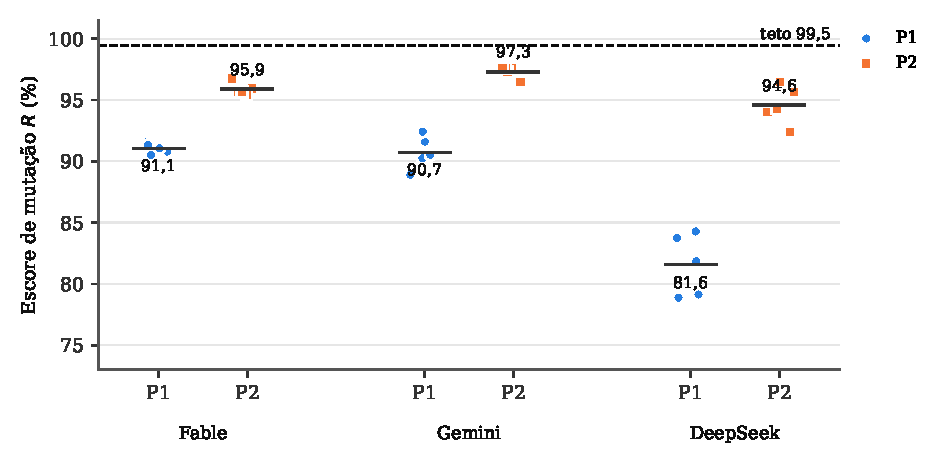
\includegraphics[width=\textwidth]{figuras/fig_r_por_condicao.pdf}
        \par
        \legend{Fonte: Própria do autor (2026).}
    \end{minipage}
\end{figure}}{\pendente{Figura: escore de mutação das cinco gerações por condição, com a linha do teto.}}

\pendente{Texto da QP1: distância média por modelo e por dimensão; destacar a diferença entre cobertura e escore de mutação. Texto da QP3: em qual dimensão a distância é maior, e se isso vale para os três modelos.}

\subsection{Efeito do prompt ciente das métricas (QP2)}

\IfFileExists{figuras/fig_gap_dimensao.pdf}{%
\begin{figure}[htb]
    \centering
    \begin{minipage}{0.9\textwidth}
        \caption{\label{fig:gap-dimensao}Distância média até o teto por dimensão, P1 e P2, por modelo}
        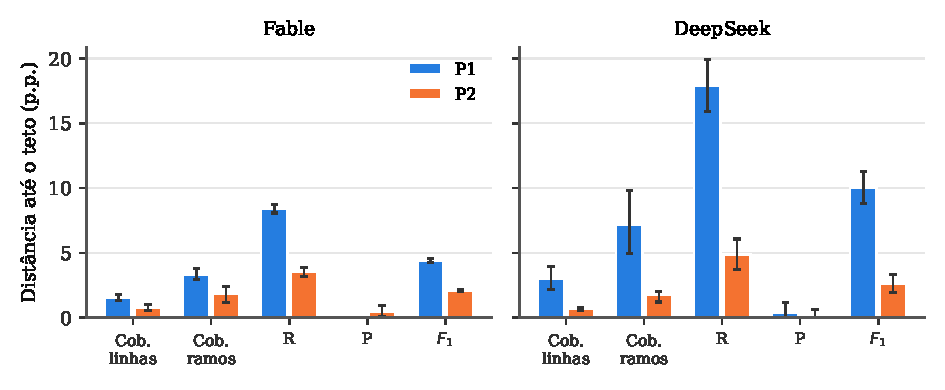
\includegraphics[width=\textwidth]{figuras/fig_gap_dimensao.pdf}
        \par
        \legend{Fonte: Própria do autor (2026).}
    \end{minipage}
\end{figure}}{\pendente{Figura: distância por dimensão, P1 vs P2, por modelo.}}

\pendente{Texto da QP2: redução média da distância com P2 por modelo e por métrica; delta de Cliff; o que mudou nas suítes (mais testes? asserções exatas? menos smells?).}

\subsection{Estabilidade entre gerações (QP4)}

\IfFileExists{tabelas/tab_estabilidade.tex}{\begin{table}[htb]
    \centering
    \ABNTEXfontereduzida
    \begin{minipage}{\textwidth}
        \caption{Estabilidade entre gerações: dispersão do escore de mutação por condição}
        \label{tab:estabilidade}
        \centering\scriptsize\setlength{\tabcolsep}{3pt}
        \begin{tabular}{ll rrr r r r r}
            \toprule
            \textbf{Condição} & \textbf{Prompt} & $\bar{R}$ & dp & CV (\%) & mín.--máx. & IC 95\% & $k^*$ & dp $F_1$ \\
            \midrule
            Fable & P1 & 91,1 & 0,4 & 0,5 & 90,5--91,6 & $\pm$0,4 & 1 & 0,2 \\
            Fable & P2 & 95,9 & 0,5 & 0,5 & 95,4--96,7 & $\pm$0,5 & 1 & 0,1 \\
            Gemini & P1 & 90,7 & 1,3 & 1,5 & 88,9--92,4 & $\pm$1,2 & 2 & 1,7 \\
            Gemini & P2 & 97,3 & 0,5 & 0,5 & 96,5--97,6 & $\pm$0,4 & 1 & 0,5 \\
            DeepSeek & P1 & 81,6 & 2,5 & 3,1 & 78,9--84,3 & $\pm$2,2 & 7 & 1,6 \\
            DeepSeek & P2 & 94,6 & 1,6 & 1,7 & 92,4--96,5 & $\pm$1,4 & 3 & 0,9 \\
            \bottomrule
        \end{tabular}
        \legend{Fonte: Própria do autor (2026). Concordância do ordenamento completo das condições por $R$ ao tomar uma geração ao acaso por condição: 49,7\% das amostras reproduzem o ordenamento pelas médias ($\tau$ médio de Kendall = 0,89). $k^*$: gerações necessárias para semi-amplitude de 2,0 p.p. no IC 95\% de $R$.}
    \end{minipage}
\end{table}
}{\pendente{Tabela de estabilidade: por condição, desvio padrão e coeficiente de variação de R e de F$_1$, amplitude (mín.--máx.), semi-amplitude do IC 95\% e $k$ necessário para semi-amplitude de 2 p.p.}}

\pendente{Texto da QP4: quanto varia; se o ordenamento das condições se mantém ao tomar uma geração ao acaso (fração de concordância); quantas gerações seriam necessárias; conclusão sobre avaliações de geração única.}

\section{Discussão}
\label{sec:discussao}

\pendente{Discussão a escrever sobre os resultados finais. Pontos já definidos pela estrutura do estudo:}

\begin{itemize}
    \item \pendente{Cobertura alta com escore de mutação menor: o que isso diz sobre as asserções geradas (relação com o problema do oráculo de \citeonline{konstantinou2024}).}
    \item \pendente{O que P2 compra e o que não compra: se o prompt fecha parte da distância, é evidência de que o modelo sabe fazer melhor quando sabe o que será medido; se não fecha, é evidência de limite de capacidade e não de informação.}
    \item \pendente{Custo: o modelo de baixo custo em relação aos de fronteira, por ponto percentual de distância.}
    \item \pendente{Se alguma geração alcançar ou superar o teto em alguma métrica: o teto é uma afirmação sobre o alvo e precisa ser revisado quando os recursos melhoram; discutir o que a suíte fez para chegar lá.}
    \item Metodológico: o achado dos \textit{timeouts} (seção ``\nameref{sec:timeout}'') vale para qualquer estudo que use Stryker ou ferramentas com limite de tempo adaptativo em execução paralela, e a revisão do teto (seção ``\nameref{sec:teto}'') mostra que ``saturou'' não é o mesmo que ``máximo''.
    \item \pendente{Implicações para a prática: usar teste de mutação como portão para testes gerados; incluir os critérios no prompt; gerar mais de uma vez e selecionar (custo de \textit{best-of-k} em relação ao ganho observado).}
\end{itemize}

\section{Ameaças à validade}
\label{sec:ameacas}

\textbf{Validade de construto.} O escore de mutação é um substituto de detecção de defeitos reais; a evidência de \citeonline{just2014} sustenta o uso, mas o acoplamento entre mutantes e defeitos reais depende do domínio. Os mutantes equivalentes permanecem no denominador para todas as suítes, o que rebaixa igualmente teto e LLMs; como os oito do teto estão classificados, o leitor pode recalcular qualquer escore na base sem equivalentes. A precisão trata cada caso de teste como um detector e um teste que falha sobre o código correto como falso positivo; essa é uma operacionalização, e outras são possíveis (por exemplo, por asserção). O catálogo de \textit{smells} do SNUTS.js não coincide um a um com o catálogo clássico de \citeonline{vandeursen2001}; medimos o que a ferramenta detecta.

\textbf{Validade interna.} O maior risco é vazamento: a LLM ver os critérios ou o teto. O aparato isola o que o modelo vê, cada geração usa uma cópia nova em caminho neutro, e memória e personalização dos aplicativos foram desligadas. A interface foi igualada entre modelos (uma mensagem, sem execução), mas não é idêntica: o modelo de ferramenta de codificação lê os arquivos por conta própria, enquanto os outros os recebem na mensagem; o conteúdo é o mesmo. A pontuação sequencial num único ambiente elimina a inflação por \textit{timeout} que afetou o piloto. O não determinismo é tratado com cinco gerações por condição, o que permite medir a dispersão, mas cinco é pouco para estimá-la com precisão; a QP4 quantifica essa limitação em vez de escondê-la.

\textbf{Validade externa.} Há um único código-alvo, pequeno, em TypeScript, com uma API de três funções e sem dependências. Os resultados não se generalizam diretamente para código com E/S, estado ou acoplamento. Os três modelos representam um recorte de novembro de 2026; versões posteriores podem mudar as distâncias. O teto é específico do alvo e precisa ser reconstruído para qualquer outro.

\textbf{Validade de conclusão.} Com cinco gerações por condição não há poder para testes de hipótese, e não os fizemos; as conclusões se apoiam em médias, intervalos por \textit{bootstrap} e tamanhos de efeito, e devem ser lidas como tal. Todos os dados brutos estão públicos para reanálise.

% ==============================================================================
% 5. CONSIDERAÇÕES FINAIS
% ==============================================================================
\chapter{Considerações finais}
\label{cap:consideracoes}

Este trabalho perguntou quão bons são os testes que uma LLM gera quando se pede a ela, numa única mensagem, que teste um módulo. Em vez de responder com cobertura ou com uma comparação contra testes humanos cuja qualidade não é medida, respondemos com a distância até um teto: a melhor suíte que conseguimos construir para o alvo, com um desenvolvedor, LLMs de fronteira e ferramentas de mutação e de \textit{smells}, e na qual cada mutante que sobrevive tem prova de que não pode ser morto. Para um avaliador de expressões com 369 mutantes, esse teto ficou em 99,5\% de escore de mutação, com cobertura de 100\% de linhas e 99,3\% de ramos, nenhum \textit{smell} e dois mutantes com prova de equivalência.

Contra esse teto, as respostas são estas. \textbf{QP1:} com o prompt básico, as suítes geradas ficam a 8,4 e 8,7 pontos percentuais do teto em escore de mutação no caso dos dois modelos de fronteira e a 17,9 no caso do modelo de baixo custo, enquanto em cobertura ficam a 3 pontos ou menos em linhas, em precisão a 2 pontos ou menos e em \textit{smells} a menos de 0,1 por teste. \textbf{QP3:} a dimensão em que a distância é maior é sempre a de detecção de defeitos, por margem de duas a sete vezes sobre a cobertura. \textbf{QP2:} informar os critérios de avaliação no prompt reduziu a distância em detecção em 57\%, 75\% e 73\%, em todas as gerações de todos os modelos, a ponto de o modelo de baixo custo orientado superar os dois modelos de fronteira sem orientação; a melhor condição, Gemini com P2, chegou a 2,2 pontos do teto; o custo foram suítes maiores e alguns falsos positivos por asserções exatas demais, dois dos quais apontavam um defeito real do alvo. \textbf{QP4:} a dispersão entre gerações depende do modelo e cai com a orientação: meio ponto nos modelos de fronteira orientados, para os quais uma geração basta, e 2,5 pontos no modelo de baixo custo com o prompt básico, para o qual seriam necessárias sete; uma geração ao acaso por condição acerta sempre as conclusões grandes (prompt, grupo de modelos) e erra entre 4\% e 36\% das vezes a ordem entre condições vizinhas.

Dois resultados valem independentemente dos números das suítes geradas. O primeiro é metodológico: pontuar mutação em paralelo inflou o escore do próprio teto em 2,4 pontos percentuais por \textit{timeouts} que não eram detecções, e essa inflação não é uniforme entre suítes, o que compromete comparações; toda pontuação com limite de tempo adaptativo deveria ser sequencial, e mutantes mortos e por \textit{timeout} deveriam ser reportados em separado. O segundo é sobre o próprio conceito de teto: uma suíte que parecia saturada ainda deixava 19 mutantes matáveis em fronteiras de classes de caracteres e em mensagens de erro, e a análise que se seguiu ainda classificou como inalcançáveis seis mutantes que uma suíte gerada depois alcançou por injeção de dependência. O que transformou a suíte em referência foi a análise individual dos sobreviventes e a revisão feita quando uma suíte gerada a superou. Uma referência de qualidade precisa de prova e de um critério explícito para ser revisada.

As limitações são as de um estudo com um alvo, três modelos e cinco gerações por condição: os números são específicos do alvo e do momento, e a dispersão foi medida com amostras pequenas. Os próximos passos seguem daí. Primeiro, repetir o protocolo em outros alvos, com características diferentes (E/S, estado, dependências), para ver se a distância e sua estrutura se mantêm. Segundo, acrescentar uma condição em que o modelo pode executar os testes e receber o resultado, para medir quanto do caminho até o teto o laço de execução fecha sozinho; se fechar quase tudo, a conclusão prática muda. Terceiro, avaliar a seleção entre várias gerações (gerar $k$ vezes e ficar com a melhor pelo escore de mutação) como estratégia de uso, com seu custo. Por fim, o aparato e o teto estão públicos e podem servir de \textit{benchmark} para modelos futuros: a distância até o teto é uma medida que não depende de quem escreveu a suíte humana de comparação, e por isso pode ser acompanhada ao longo do tempo.


% ==========================================================================
% ELEMENTOS PÓS-TEXTUAIS
% ==========================================================================
\postextual


% --- Referências bibliográficas ---
\bibliography{referencias}
\newpage



% --- Apêndices ---
\begin{apendicesenv}
    % %Imprime uma página indicando o início dos apêndices
    % \partapendices

    % ==============================================================================
% APÊNDICE A — PROMPTS
% ==============================================================================

\section{Prompts utilizados}
\label{ap:prompts}

Os dois prompts foram usados exatamente como abaixo, em inglês, em todas as condições. P2 é P1 acrescido da seção \textit{Quality criteria}. Para os modelos sem acesso ao sistema de arquivos, a mensagem continha, após o prompt, uma seção \textit{Files} com o conteúdo de \texttt{package.json}, \texttt{vitest.config.ts} e dos cinco arquivos de \texttt{src/}, cada um em um bloco de código identificado pelo caminho.

\subsection*{P1 -- prompt básico}

\begin{lstlisting}[language={}, caption={Prompt P1}, label={lst:p1}]
# Task

Write unit tests for the expression parser in `src/`.

Its public API is `evaluate(expression, context?)` and
`evaluateObject(expression, value)` in `src/evaluator.ts`,
plus `parse(expression)` in `src/parser.ts`.

Use Vitest. Put the tests in `tests/expression-parser.test.ts`.

You can run `pnpm test` to execute the tests.
\end{lstlisting}

\subsection*{P2 -- prompt ciente das métricas}

\begin{lstlisting}[language={}, caption={Prompt P2 (acréscimo a P1)}, label={lst:p2}]
[... texto de P1 ...]

## Quality criteria

The tests will be evaluated along three dimensions. Aim to
maximize them:

1. **Code coverage** - exercise every line, branch, and
   condition of the code under test.
2. **Fault-detection power** - the tests must fail if the
   code's behavior changes. Assert exact return values and
   test boundary cases (values at the edge of the conditions,
   and just above/below the edge), so that small changes in
   the logic are detected.
3. **Maintainability** - avoid test smells. In particular: do
   not pile up many assertions without messages in a single
   test (Assertion Roulette); do not duplicate the same
   assertion; each test should cover a single behavior (avoid
   Eager Test); avoid unexplained magic numbers; and do not
   depend on external resources or shared state between tests.
\end{lstlisting}

    \newpage
    % ==============================================================================
% APÊNDICE B — MUTANTES EQUIVALENTES DO TETO
% ==============================================================================

\section{Mutantes que restam vivos no teto}
\label{ap:equivalentes}

A suíte do teto mata 367 dos 369 mutantes válidos (338 por falha de asserção e 29 por \textit{timeout} legítimo). O \autoref{qua:equivalentes} registra, para cada um dos dois restantes, o argumento de por que nenhum teste pode distingui-lo do programa original, e o \autoref{qua:revisao2} registra os seis mutantes que uma primeira análise havia classificado como inalcançáveis e que a segunda revisão matou por injeção de dependência. O registro completo, com o censo do Stryker e o histórico das revisões, está no arquivo \texttt{runs/ceiling/EQUIVALENT\_MUTANTS.md} do repositório.

\begin{quadro}[htb]
    \centering
    \ABNTEXfontereduzida
    \begin{minipage}{\textwidth}
        \caption{Mutantes equivalentes do teto}
        \label{qua:equivalentes}
        \centering
        \begin{tabular}{p{0.5cm}p{2.6cm}p{3.8cm}p{7.9cm}}
            \toprule
            \textbf{\#} & \textbf{Local} & \textbf{Mutação} & \textbf{Por que nenhum teste distingue} \\
            \midrule
            1 & \texttt{lexer.ts:12} & \texttt{currentChar = '\textbackslash 0'} $\to$ \texttt{""} & Inicializador morto: o construtor chama \texttt{readChar()} imediatamente, que reatribui o campo em todos os caminhos antes de qualquer leitura. O campo é privado e nunca é lido antes dessa reatribuição, então nem injeção o alcança. \\
            2 & \texttt{lexer.ts:109} & \texttt{peekChar()} devolve \texttt{""} em vez de \texttt{'\textbackslash 0'} no fim da entrada & O valor só é usado em comparações com \texttt{'>'} e \texttt{'='} e nos classificadores \texttt{isLetter}, \texttt{isNumber} e \texttt{isDot}. \texttt{"".charCodeAt(0)} é \texttt{NaN} e \texttt{'\textbackslash 0'.charCodeAt(0)} é 0; ambos falham em todas as comparações de faixa, e nenhum dos dois é \texttt{'.'}, \texttt{'>'} ou \texttt{'='}. O método é privado e seu retorno nunca escapa da classe. \\
            \bottomrule
        \end{tabular}
        \legend{Fonte: Própria do autor (2026).}
    \end{minipage}
\end{quadro}

\begin{quadro}[htb]
    \centering
    \ABNTEXfontereduzida
    \begin{minipage}{\textwidth}
        \caption{Mutantes classificados como inalcançáveis na primeira análise e mortos na segunda revisão}
        \label{qua:revisao2}
        \centering
        \begin{tabular}{p{0.7cm}p{3.0cm}p{4.2cm}p{6.9cm}}
            \toprule
            \textbf{\#} & \textbf{Local} & \textbf{Mutação} & \textbf{Teste que o mata} \\
            \midrule
            3--4 & \texttt{evaluator.ts:47--48} & ramo \texttt{default} do \texttt{switch} de operadores binários e sua mensagem & \texttt{parse} envolvido com \texttt{vi.mock} devolve, uma vez, \texttt{BinaryExpression(Not, 1, 2)}; \texttt{evaluate} deve lançar \texttt{Operator not not implemented}. \\
            5--6 & \texttt{evaluator.ts:77--78} & ramo \texttt{default} do \texttt{switch} de tipos de nó e sua mensagem & \texttt{parse} devolve, uma vez, \texttt{UnaryExpression(Minus, 1)}; \texttt{evaluate} deve lançar \texttt{Invalid AST node}. \\
            7--8 & \texttt{parser.ts:143--144} & bloco do \texttt{if (!this.expectPeekToken(Rparn))} e sua mensagem & \texttt{vi.spyOn} em \texttt{Parser.prototype.expectPeekToken} devolve \texttt{undefined} uma vez; \texttt{parse('(1)')} deve lançar \texttt{Expected ) but got \ldots}. \\
            \bottomrule
        \end{tabular}
        \legend{Fonte: Própria do autor (2026).}
    \end{minipage}
\end{quadro}

\end{apendicesenv}

% --- Índice remissivo (opcional) ---
% \phantompart
% \printindex

\end{document}
